\Chapter{Több étterem, egy futár, több kiszállítás esete}

\Section{A probléma megfoglmazása}

Több étterem esetén meg kell határozni néhány feltételt. Jelen helyzetben a futár elindul az egyik étteremből, kiszállít mindent, majd egy másik étterembe érkezik ezt követően, és annak a rendeléseit is kiszállítja. Időben is meg kell szabni néhány határt, miszerint az első étteremből való indulás pillanatáig beérkezett rendeléseket szállítja csak ki az összes étteremből. Miután sikeresen kivitte az összes rendelést visszatér a kezdő étterembe és kezdődik előlről a folyamat. Maga a folyamat egy önmagát ismételő klasszikus utazó ügynök probléma, annyi eltéréssel, hogy nem ugyan abba az étterembe kell érkeznie ahonnan indult, hanem a hozzá legközelebb esőbe amelyikbe még nem járt az adott ciklusban. A probléma szemléltetése \aref{fig:model3}. ábrán látható.

\begin{figure}[h!]
\centering
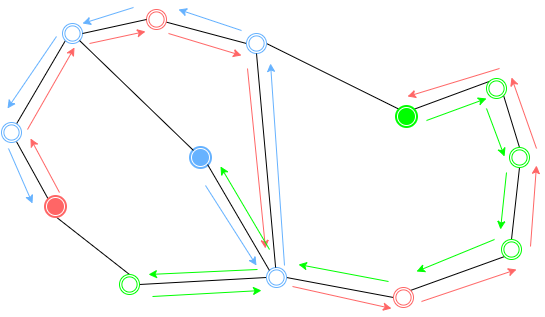
\includegraphics[scale=0.6]{images/Circulartsp.png}
\caption{Több étterem, egy futár, több kiszállítás modellje}
\label{fig:model3}
\end{figure}


\Section{A probléma megoldása}

Maga a probléma egy már megoldott helyzetre vezethető vissza. Az egy étterem, egy futár, több kiszállítás eseténél mindig ugyanabba az egy étterembe kellett visszatérnie a futárnak. Az ott alkalmazott módszerek érvényesek erre az esetre is, annyi eltéréssel, hogy ha kiszállította egy étterem rendeléseit az utolsó megállóhelye a folyamatban a következő étterem (nem az amiből indult). A folyamat következő lépése pedig innen indul, a futár kiszállítja az összes rendelést és egy harmadik étterembe érkezik utolsóképp. Ez mindaddig tart, amíg a futár meg nem látogatja az összes éttermet és vissza nem tér a kezdő, kiinduló étterembe. 

\Section{A megoldás implementálása}

Az előző megoldást felhasználva, pár változtatást el kellett végezni, hogy helyesen működjön erre az esetre.

Be kellett vezetni egy összegzést ami az éttermek számát határozza meg.
\begin{python}
restaurantCount = 4
\end{python}
Ezt követően feltöltöttem egy listát véletlenszerűen generált $x$ és $y$ koordinátákkal. Maga a lista hossza az előbb meghatározott \texttt{restaurantCount}-al egyenlő.
\begin{python}
restaurants = [random.sample(range(100),2)
               for x in range(restaurantCount)] 
\end{python}
Szükségszerű volt bevezetni egy külső ciklust, ami az éttermek számáig megy. Ezáltal nyerhetőek vissza az adott étterem koordinátái.
\begin{python}
for l in range(len(restaurants)):
\end{python}
A cikluson belül a pontok számát csökkentenünk kellett egyel, valamint az első helyre hozzáadni a \texttt{restaurants} adott \texttt{l} elemét. Ezáltal meg van oldva, hogy a ciklus mindig az éttermektől induljon.

\begin{python}
travel = [random.sample(range(100), 2) for x in range(pointCount - 1)]
travel.insert(0, restaurants[l])
\end{python}

Meg kell még oldani, hogy a ciklus utolsó eleme a következő étterem koordinátája legyen. Figyelembe kellett venni azt is, hogy az utolsó étterem utolsó pontja az első étterem koordinátáival kell, hogy megegyezzenek. Szükségessé vált a kör megszakítása is a gráfban. 
Ezek a következőképpen néznek ki. 
\begin{python}
helperX = travel[i % pointCount]][0] for i in range(pointCount)
helperY = travel[i % pointCount]][1] for i in range(pointCount)

if l < (len(restaurants) - 1):
	helperX.append(restaurants[l+1][0])
	helperY.append(restaurants[l+1][1])
else:
	helperX.append(restaurants[0][0])
	helperX.append(restaurants[0][1])
\end{python}

\Section{A megoldás tesztelése}

A módszer vizsgálatához 4 éttermet és 36 kiszállítási helyet vettem számításba.
Az elkészített program által visszaadott útvonalak \aref{fig:tspMR1}., \ref{fig:tspMR2}., \ref{fig:tspMR3}.  és \ref{fig:tspMR4}. ábrán láthatók.
Jól megfigyelhető, hogy az utolsó étterem utolsó pontja visszatér az első étterem koordinátáihoz a (71, 42) pontba.

\begin{figure}[h!]
\centering
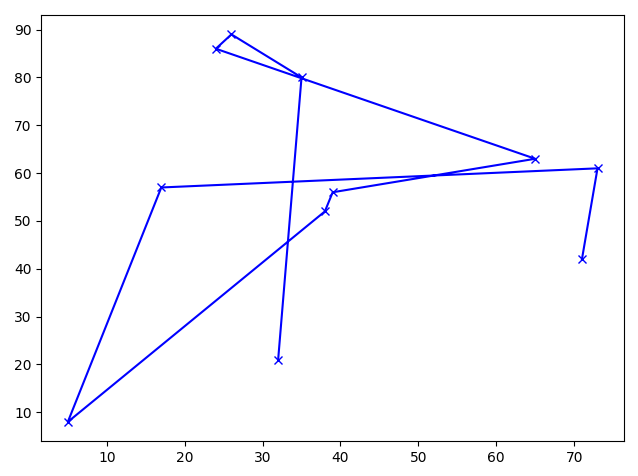
\includegraphics[scale=0.8]{images/tsp1MR.png}
\caption{Első étterem poziciója: (71, 42)}
\label{fig:tspMR1}
\end{figure}

\begin{figure}[h!]
\centering
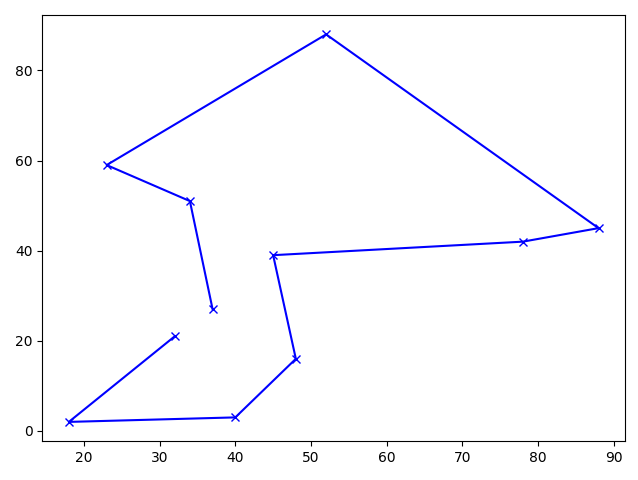
\includegraphics[scale=0.8]{images/tsp2MR.png}
\caption{Második étterem poziciója: (32, 21)}
\label{fig:tspMR2}
\end{figure}

\begin{figure}[h!]
\centering
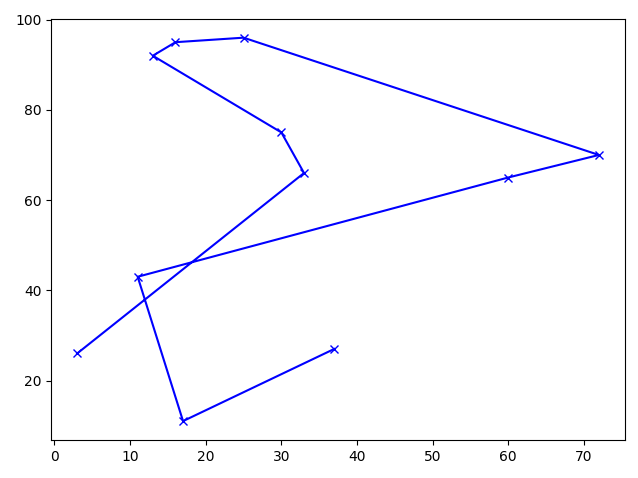
\includegraphics[scale=0.8]{images/tsp3MR.png}
\caption{Harmadik étterem poziciója: (37, 27)}
\label{fig:tspMR3}
\end{figure}

\begin{figure}[h!]
\centering
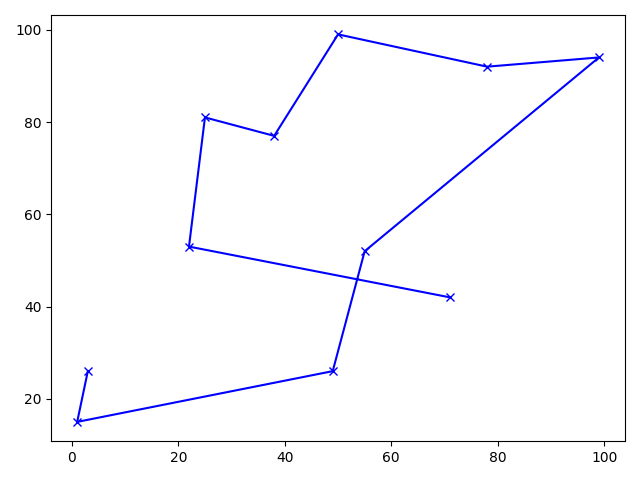
\includegraphics[scale=0.8]{images/tsp4MR.png}
\caption{Negyedik étterem poziciója: (3, 26)}
\label{fig:tspMR4}
\end{figure}